% partes/parte2/cap06.tex
\chapter{El proceso de decisión de compra}
\label{cap:06}

\begin{cajaFicha}
\begin{description}
  \item[Unidad temática] II — Proceso de toma de decisión de compra digital.
  \item[Temas del programa] 2.1 Proceso de toma de decisiones de compra: 2.1.1 Reconocimiento de necesidades y/o deseos; 2.1.2 Búsqueda de información; 2.1.3 Evaluación de alternativas; 2.1.4 Decisión de compra-consumo; 2.1.5 Evaluación post-compra-satisfacción.
  \item[Horas] Teoría 2.0 · Práctica 4.0 · Aprendizaje autónomo 2.0 (asignación tentativa; ver Anexo B del prompt de proyecto, anomalía 4).
  \item[Competencia de la unidad] Examina el proceso de toma de decisiones de compra del consumidor digital a partir de su recorrido y figuras participantes.
  \item[Resultados de aprendizaje observables] Al concluir el capítulo, el estudiante:
  \begin{enumerate}
    \item describe las cinco etapas del proceso de decisión y distingue qué cambia en cada una cuando el entorno es digital;
    \item diferencia una regla compensatoria de una no compensatoria y predice cuándo darán elecciones distintas;
    \item explica la diferencia entre un \textit{nudge} y un patrón oscuro con un criterio verificable;
    \item aplica tres reglas de decisión a un mismo conjunto de alternativas y localiza el peso a partir del cual cambia la elección.
  \end{enumerate}
  \item[Prerrequisitos] Cap. 1--5.
\end{description}
\end{cajaFicha}

\section{Caso de apertura}

\begin{casoFicticio}
Mariana necesita audífonos inalámbricos. A las once de la noche recibe una
notificación: \enquote{Quedan 2 piezas. Tu carrito expira en 10 minutos}.
No había abierto la aplicación en toda la semana. Compra. A la mañana
siguiente descubre que el modelo que eligió tardará siete días en llegar y
que otro, de precio similar, llegaba en dos.

Las preguntas son simples. ¿Mariana \emph{reconoció} una necesidad o se la
fabricaron? ¿Evaluó alternativas o solo reaccionó al temporizador? ¿Qué parte
de la decisión fue suya?
\end{casoFicticio}

El caso es ficticio, pero el patrón es real. El proceso de decisión de compra
es un modelo de cinco etapas que los libros de texto describen como un
recorrido ordenado. En el entorno digital ese orden se rompe: el algoritmo
puede disparar la primera etapa, el temporizador puede comprimir la tercera y
la reseña puede convertir la quinta en la primera de otro consumidor. Este
capítulo explica el modelo, muestra dónde se tuerce en internet y entrega una
herramienta para analizarlo: tres reglas de decisión que, aplicadas a los
mismos datos, pueden elegir tres productos distintos.

\section{Desarrollo teórico}

El esquema de cinco etapas procede de la tradición de procesamiento de
información del comportamiento del consumidor. Los tres textos de la
bibliografía oficial lo usan como columna vertebral, con matices de
formulación \parencite{solomon2023consumer,hoyer2024consumer,kotler2021marketing50}.
La figura~\ref{fig:cap06-proceso} lo resume y marca las dos variantes que el
entorno digital introduce.

\begin{figure}[!htb]
  \centering
  \resizebox{\textwidth}{!}{% figuras/tikz/cap06-proceso-decision.tex
% Proceso de decisión de compra en cinco etapas, con las dos variantes digitales
% que el capítulo discute: reconocimiento inducido y bucle de reseñas.
\begin{tikzpicture}[
    etapa/.style={rectangle, rounded corners, draw=guindaIPN, thick, fill=guindaIPNClara,
                  minimum width=2.55cm, minimum height=1.35cm, align=center, font=\scriptsize},
    flecha/.style={-{Stealth[length=2.5mm]}, thick, draw=doradoIPN},
    nota/.style={font=\tiny, text=grisIPN, align=center}
  ]
  \node[etapa] (e1) at (0,0)    {\textbf{2.1.1}\\ Reconocimiento de\\ necesidad o deseo};
  \node[etapa] (e2) at (3.0,0)  {\textbf{2.1.2}\\ Búsqueda de\\ información};
  \node[etapa] (e3) at (6.0,0)  {\textbf{2.1.3}\\ Evaluación de\\ alternativas};
  \node[etapa] (e4) at (9.0,0)  {\textbf{2.1.4}\\ Decisión de\\ compra-consumo};
  \node[etapa] (e5) at (12.0,0) {\textbf{2.1.5}\\ Evaluación\\ post-compra};
  \foreach \a/\b in {e1/e2,e2/e3,e3/e4,e4/e5} { \draw[flecha] (\a) -- (\b); }

  % variante digital 1: el disparador puede venir del algoritmo
  \node[nota] (ind) at (0,2.1) {notificación, recomendación\\ algorítmica, \textit{retargeting}};
  \draw[flecha, draw=terracotaIPN, dashed] (ind) -- (e1);
  \node[nota, text=terracotaIPN] at (0,3.0) {reconocimiento inducido};

  % retroceso típico de la fase de evaluación
  \draw[flecha, draw=bronceIPN, dashed] (e3.north) to[bend right=40] node[above, nota, text=bronceIPN] {se vuelve a buscar} (e2.north);

  % variante digital 2: la reseña propia alimenta la búsqueda de otros
  \draw[flecha, draw=bronceIPN, dashed] (e5.south) -- ++(0,-1.0) -| node[below, pos=0.25, nota, text=bronceIPN] {reseña, calificación y \textit{unboxing} alimentan la búsqueda de otros consumidores} (e2.south);
\end{tikzpicture}
}
  \caption{Proceso de decisión de compra en cinco etapas y sus dos variantes
  digitales (reconocimiento inducido y bucle de reseñas). Fuente: elaboración
  propia a partir del esquema de cinco etapas de los textos de la bibliografía
  oficial.}
  \label{fig:cap06-proceso}
\end{figure}

\subsection{Reconocimiento de necesidades y/o deseos}
\progtag{2.1.1}

En el modelo clásico, la decisión empieza con una brecha: el consumidor
percibe una distancia entre su estado actual y el que desea. La brecha puede
ser una necesidad (se acabó el café) o un deseo (quiero otro teléfono aunque
el mío funcione).

Internet añade una variante que el modelo original no contemplaba: el
\emph{reconocimiento inducido}. Una notificación, una recomendación
algorítmica o un anuncio de \textit{retargeting} generan una necesidad
percibida sin que exista una carencia funcional previa. El mecanismo es
distinto, aunque la etapa lleve el mismo nombre. En el clásico, la brecha
nace en la persona. En el inducido, nace en el diseño del canal. Lo anterior
no vuelve ilegítimo el recordatorio, pero obliga a preguntar quién decidió
que había una brecha.

\subsection{Búsqueda de información}
\label{sec:cap06-busqueda}
\progtag{2.1.2}

La búsqueda digital mezcla tres tipos de fuente: las que controla la marca
(sitio propio, correo), las de terceros (buscadores, comparadores, reseñas) y
las sociales (recomendaciones de pares, contenido generado por usuarios). El
consumidor no recorre las tres en orden. Salta de una a otra según la
categoría y el riesgo percibido.

Dos conductas ilustran esa mezcla. El \textit{webrooming} consiste en
investigar en línea y comprar en tienda física. El \textit{showrooming} es la
inversa: probar en tienda y comprar en línea. La revisión bibliométrica de
\textcite{halibas2023showrooming} confirma que ambas coexisten y que dependen
de la categoría de producto, no de un tipo fijo de consumidor. La
consecuencia práctica es clara: asignar a una persona la etiqueta
\enquote{comprador en línea} describe una compra, no una identidad.

\subsection{Evaluación de alternativas}
\label{sec:cap06-evaluacion}
\progtag{2.1.3}

Aquí el modelo económico clásico supone que el consumidor pondera todos los
atributos de todas las alternativas y elige la de mayor utilidad. Casi nadie
decide así. \textcite{simon1955} propuso que las personas, con tiempo y
atención limitados, buscan una opción \enquote{suficientemente buena} y no la
óptima. \textcite{payne1988adaptive} mostraron después que quien decide
cambia de estrategia según el esfuerzo que cada una exige: ante muchas
alternativas, descarta primero y compara después.

Esa distinción organiza el laboratorio del capítulo. Las reglas se agrupan en
dos familias (figura~\ref{fig:cap06-reglas}):

\begin{figure}[!htb]
  \centering
  \resizebox{0.82\textwidth}{!}{% figuras/tikz/cap06-reglas-decision.tex
% Reglas compensatorias y no compensatorias de evaluación de alternativas.
\begin{tikzpicture}[
    regla/.style={rectangle, rounded corners, draw=guindaIPN, thick, fill=guindaIPNClara,
                  minimum width=4.6cm, minimum height=1.9cm, align=center, font=\scriptsize},
    nocomp/.style={rectangle, rounded corners, draw=bronceIPN, thick, fill=bronceIPNClaro,
                   minimum width=4.6cm, minimum height=1.9cm, align=center, font=\scriptsize},
    centro/.style={rectangle, draw=grisIPN, thick, fill=white, minimum width=3.2cm, minimum height=1.2cm, align=center, font=\small\bfseries},
    flecha/.style={-{Stealth[length=2.5mm]}, thick, draw=doradoIPN}
  ]
  \node[regla]  (a) at (0,3.0)  {\textbf{Aditiva ponderada}\\ \textit{compensatoria}\\ suma puntaje $\times$ peso;\\ lo bueno compensa lo malo};
  \node[nocomp] (b) at (0,0.5)  {\textbf{Conjuntiva}\\ \textit{no compensatoria}\\ cada atributo debe superar\\ un mínimo; si no, se descarta};
  \node[nocomp] (c) at (0,-2.0) {\textbf{Lexicográfica}\\ \textit{no compensatoria}\\ manda el atributo más importante;\\ el siguiente solo desempata};
  \node[centro] (d) at (7.0,0.5) {Alternativa\\ elegida};
  \foreach \n in {a,b,c} { \draw[flecha] (\n.east) -- (d.west); }
  \node[font=\tiny, text=grisIPN, align=center] at (3.5,-3.6) {Los mismos datos pueden producir tres elecciones distintas.};
\end{tikzpicture}
}
  \caption{Reglas compensatorias y no compensatorias de evaluación de
  alternativas. Fuente: elaboración propia.}
  \label{fig:cap06-reglas}
\end{figure}

\begin{table}[!htb]
\centering
\begin{tabular}{@{}p{2.8cm}p{3.5cm}p{6.2cm}@{}}
\toprule
Regla & Familia & Cómo decide \\
\midrule
Aditiva ponderada & Compensatoria & Multiplica el puntaje de cada atributo por su peso y suma. Un atributo excelente puede tapar uno malo. \\
Conjuntiva & No compensatoria & Fija un mínimo por atributo. Quien falla en uno solo queda fuera, sin importar lo demás. \\
Lexicográfica & No compensatoria & Ordena los atributos por importancia. Decide el primero; el siguiente solo desempata cuando la diferencia cae dentro de una tolerancia. \\
\bottomrule
\end{tabular}
\caption{Tres reglas de decisión usadas en el laboratorio. Fuente: elaboración
propia con base en \textcite{payne1988adaptive}.}
\label{tab:cap06-reglas}
\end{table}

Sobre esto último, \textcite{tverskykahneman1974} documentaron que las
personas recurren a heurísticas (atajos de juicio) cuando la información es
abundante o incierta. Las más estudiadas son la representatividad, la
disponibilidad y el anclaje. En internet, la interfaz puede activarlas o
mitigarlas. El recuadro de Frontera de esta sección desarrolla el punto.

\begin{cajaFrontera}
\textbf{Economía conductual aplicada: del \textit{nudge} al patrón oscuro.}
\textcite{thaler2003libertarian} y \textcite{thalersunstein2008} trasladaron
los hallazgos de las heurísticas al diseño de \emph{arquitecturas de
elección}. Un \textit{nudge} modifica el contexto de la decisión sin
prohibir opciones ni cambiar de forma significativa los incentivos
económicos; la libertad de elegir queda intacta.

Una tienda en línea es, literalmente, una arquitectura de elección. El orden
de los resultados, la insignia de \enquote{más vendido}, el temporizador y el
pago en un clic son decisiones de diseño. \textcite{mathur2019} rastrearon
11\,000 sitios de compra y documentaron cómo esas mismas palancas
(urgencia, escasez, prueba social) se usan para acelerar la decisión y
reducir la comparación real. \textcite{luguristrahilevitz2021} midieron el
efecto en dos experimentos con muestras representativas de consumidores
estadounidenses: quienes vieron patrones oscuros leves tuvieron más del doble
de probabilidad de conservar un servicio que no habían pedido, y quienes
vieron patrones agresivos, casi cuatro veces.

El criterio que separa ambos casos es verificable. Un \textit{nudge} usa
información veraz y deja una salida igual de fácil que la entrada. Un patrón
oscuro miente sobre la urgencia, esconde la salida o hace costosa la
negativa (cuadro~\ref{tab:cap06-nudge}, figura~\ref{fig:cap06-nudge}). En
Europa, el informe del Parlamento Europeo \parencite{eprs2025darkpatterns}
sintetiza el debate regulatorio; en México, el tema se retoma en los
capítulos sobre factores psicológicos.
\end{cajaFrontera}

\begin{figure}[!htb]
  \centering
  \resizebox{0.85\textwidth}{!}{% figuras/tikz/cap06-nudge-dark.tex
% Del \textit{nudge} al patrón oscuro: la misma heurística, dos arquitecturas de elección.
\begin{tikzpicture}[
    caja/.style={rectangle, rounded corners, draw=guindaIPN, thick, fill=guindaIPNClara,
                 minimum width=4.4cm, minimum height=1.6cm, align=center, font=\scriptsize},
    cajaA/.style={rectangle, rounded corners, draw=terracotaIPN, thick, fill=terracotaIPNClara,
                  minimum width=4.4cm, minimum height=1.6cm, align=center, font=\scriptsize},
    flecha/.style={-{Stealth[length=2.5mm]}, thick, draw=doradoIPN}
  ]
  \node[caja,  anchor=east] (n) at (-0.6,0) {\textbf{Nudge}\\ preserva la libertad\\ de elección informada};
  \node[cajaA, anchor=west] (d) at (0.6,0)  {\textbf{Patrón oscuro}\\ erosiona la elección\\ informada a propósito};
  \node[font=\small\bfseries, align=center] (h) at (0,3.0) {Heurística:\\ urgencia, escasez, prueba social};
  \draw[flecha] (h) -- ++(0,-0.9) -| (n.north);
  \draw[flecha, draw=terracotaIPN] (h) -- ++(0,-0.9) -| (d.north);
  \draw[-{Stealth[length=2.5mm]}, thick, draw=grisIPN] (-5.2,-1.6) -- (5.2,-1.6);
  \node[font=\tiny, text=grisIPN, anchor=east] at (-4.9,-2.0) {información veraz, salida fácil};
  \node[font=\tiny, text=grisIPN, anchor=west] at (4.9,-2.0) {falsa urgencia, salida difícil};
\end{tikzpicture}
}
  \caption{La misma heurística puede alimentar un \textit{nudge} o un patrón
  oscuro. Fuente: elaboración propia a partir de \textcite{thalersunstein2008}
  y \textcite{mathur2019}.}
  \label{fig:cap06-nudge}
\end{figure}

\begin{table}[!htb]
\centering
\begin{tabular}{@{}p{2.6cm}p{4.9cm}p{5.0cm}@{}}
\toprule
Palanca & \textit{Nudge} (ejemplo) & Patrón oscuro (ejemplo) \\
\midrule
Escasez & Muestra el inventario real cuando queda poco. & Anuncia \enquote{quedan 2} con un número fijo que nunca baja. \\
Urgencia & Informa la fecha real en que termina una promoción. & Temporizador que se reinicia al recargar la página. \\
Prueba social & Muestra la calificación promedio con el total de reseñas. & Notificaciones de \enquote{alguien compró esto} generadas al azar. \\
Salida & Cancelar cuesta lo mismo que contratar. & Contratar toma un clic; cancelar exige llamar por teléfono. \\
\bottomrule
\end{tabular}
\caption{Contraste entre \textit{nudge} y patrón oscuro, por palanca. Los
ejemplos son ilustrativos; la taxonomía empírica completa está en
\textcite{mathur2019}. Fuente: elaboración propia.}
\label{tab:cap06-nudge}
\end{table}

\subsection{Decisión de compra-consumo}
\progtag{2.1.4}

La decisión se concreta en el pago. Aquí pesa la fricción: cuántos pasos exige
el \textit{checkout}, qué medios de pago acepta, cuándo aparece el costo de
envío. El modelo lineal suele omitir que muchos consumidores llegan a este
punto y regresan a evaluar al menos una vez. \textcite{court2009consumer}
documentaron ese retroceso hace más de quince años, y el Cap.~7 lo desarrolla
como crítica al embudo lineal.

Conviene separar dos eventos que el lenguaje cotidiano mezcla. \emph{Comprar}
es transferir el pago. \emph{Consumir} es usar el producto o servicio. La
satisfacción depende del segundo, no del primero.

\subsection{Evaluación post-compra y satisfacción}
\progtag{2.1.5}

Después de consumir, el cliente compara su experiencia con lo que esperaba.
Si el desempeño iguala o supera la expectativa, hay satisfacción; si no,
disonancia o queja. El canal digital amplifica esta etapa porque la vuelve
pública. La calificación, la reseña y el video de desempaque se convierten en
información para la etapa 2.1.2 de otros consumidores. El proceso deja de ser
una línea y se vuelve un bucle (figura~\ref{fig:cap06-proceso}), razón
adicional para estudiar el recorrido completo en el capítulo siguiente.

\section{Evidencia de México y del mundo}

El contexto cuantitativo importa para dimensionar el fenómeno, no para
adornarlo. Según la ENDUTIH 2025, 86.1\,\% de la población de seis años o más
usó internet en México, y 37.3\,\% de las personas usuarias reportó haber
comprado en línea \parencite{inegi2026endutih}. Por el lado de la oferta, el
estudio de la Asociación Mexicana de Venta Online estima que el comercio
electrónico minorista alcanzó 941 mil millones de pesos en 2025, con un
crecimiento anual de 19.2\,\%, una participación de 17.7\,\% en las ventas
minoristas y 77.2 millones de compradores digitales \parencite{amvo2026}.

\begin{table}[!htb]
\centering
\begin{tabular}{@{}p{5.6cm}p{2.4cm}p{4.5cm}@{}}
\toprule
Indicador (México, 2025) & Cifra & Fuente \\
\midrule
Población de 6 años o más usuaria de internet & 86.1\,\% & ENDUTIH 2025 \parencite{inegi2026endutih} \\
Personas usuarias de internet que compraron en línea & 37.3\,\% & ENDUTIH 2025 \parencite{inegi2026endutih} \\
Valor del comercio electrónico minorista & 941 mil millones de pesos & AMVO, Estudio de Venta Online 2026 \parencite{amvo2026} \\
Participación del comercio electrónico en ventas minoristas & 17.7\,\% & AMVO 2026 \parencite{amvo2026} \\
Compradores digitales & 77.2 millones & AMVO 2026 \parencite{amvo2026} \\
\bottomrule
\end{tabular}
\caption{Dimensión del comercio digital en México. Las dos fuentes miden
cosas distintas (encuesta a hogares, estudio gremial) y no deben sumarse ni
compararse como si fueran la misma base. Fuente: ver columna.}
\label{tab:cap06-mexico}
\end{table}

Una lectura cuidadosa de este cuadro evita un error frecuente. Que 37.3\,\% de
las personas usuarias haya comprado en línea no significa que 62.7\,\% decida
\enquote{fuera} del entorno digital. Quien no compró en línea pudo haber
investigado en línea y pagar en tienda. Es el \textit{webrooming} de la
sección~\ref{sec:cap06-busqueda}: la compra no ocurre en internet, pero la decisión sí pasó por él.

\section{Laboratorio MATLAB: tres reglas de decisión sobre las mismas alternativas}
\label{sec:cap06-lab}

\begin{cajaLaboratorio}
\textbf{Objetivo.} Aplicar la regla aditiva ponderada, la conjuntiva y la
lexicográfica a seis alternativas \textbf{ficticias} de un mismo producto,
comparar la elección de cada una y localizar el peso del precio a partir del
cual cambia la decisión.

\textbf{Concepto detrás del código.} Cada atributo tiene unidades distintas
(pesos, días, estrellas). Para compararlos se lleva a una escala común de 0 a
10 con \emph{min-max}: si $x_{ij}$ es el valor de la alternativa $i$ en el
atributo $j$,
\[
  s_{ij} = 10\,\frac{x_{ij}-\min_i x_{ij}}{\max_i x_{ij}-\min_i x_{ij}},
\]
y en los atributos de costo (precio, días de entrega) se invierte, $s_{ij}
\leftarrow 10 - s_{ij}$, para que 10 siempre signifique \enquote{lo mejor}. La
regla aditiva calcula la utilidad $U_i=\sum_j w_j\,s_{ij}$, con pesos
$w_j\ge 0$ normalizados para sumar 1. La conjuntiva conserva solo las
alternativas con $s_{ij}\ge u$ en \emph{todos} los atributos y elige, entre
ellas, la de mayor $U_i$. La lexicográfica recorre los atributos por orden de
importancia: en cada uno conserva a las alternativas que quedan a menos de la
tolerancia $\tau$ de la mejor, y se detiene cuando queda una.

\textbf{Script.} \texttt{matlab/cap06/cap06\_alternativas.m}. Es el
\textbf{mismo script, sin modificar}, que se usa en la práctica única
\enquote{Recorrido del consumidor digital} de esta Parte. Los datos son
\textbf{sintéticos}: las marcas (Alfa, Beta\ldots) y sus atributos son
inventados, y no representan producto ni mercado alguno. No hay números
aleatorios; el resultado es idéntico en cada corrida.

\begin{lstlisting}[style=MATLABStyle, caption={Bloque de parámetros editable (\texttt{cap06\_alternativas.m}) — es lo único que cambia entre corridas.}]
pesoPrecio = 0.40;          % importancia del precio (>= 0; se normalizan)
pesoCalidad = 0.30;         % importancia de la calidad percibida
pesoEntrega = 0.15;         % importancia de la rapidez de entrega
pesoResenas = 0.15;         % importancia de las resenas
umbralMinimo = 3.5;         % regla conjuntiva: minimo (0 a 10) en CADA atributo
atributoPrioritario = 2;    % regla lexicografica: 1 precio, 2 calidad, 3 entrega, 4 resenas
toleranciaLex = 0.5;        % regla lexicografica: diferencia que cuenta como empate
\end{lstlisting}

\textbf{Salida esperada.} Dos figuras: la utilidad aditiva de cada alternativa
con la elección de cada regla (figura~\ref{fig:cap06-reglas-decision}) y la
sensibilidad al peso del precio (figura~\ref{fig:cap06-sensibilidad}).

\begin{center}
  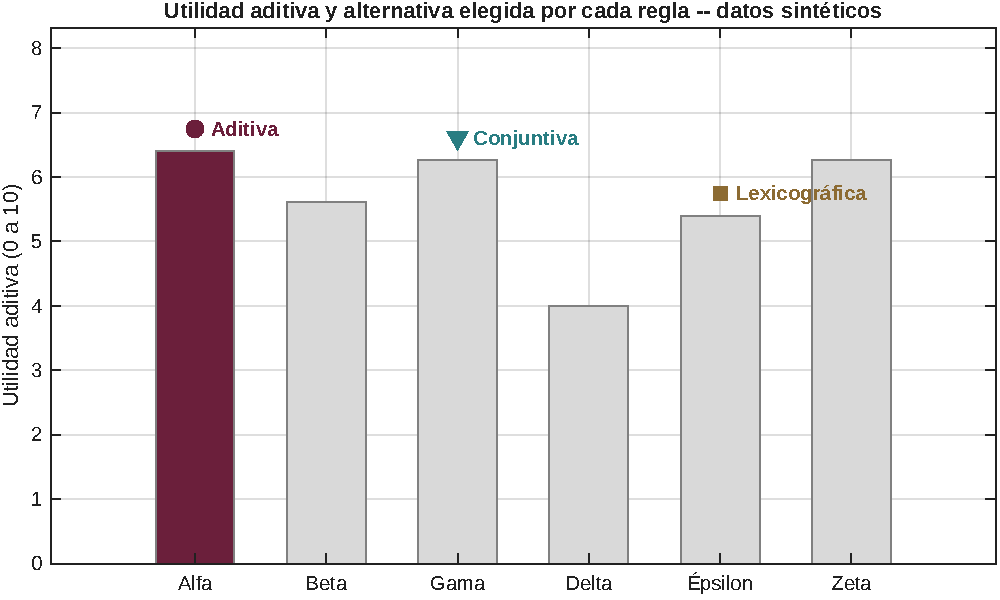
\includegraphics[width=0.88\textwidth]{figuras/matlab/cap06_reglas_decision.pdf}
  \captionof{figure}{Utilidad aditiva y alternativa elegida por cada regla con
  los parámetros por defecto. Fuente: elaboración propia con datos sintéticos.}
  \label{fig:cap06-reglas-decision}
\end{center}

\begin{center}
  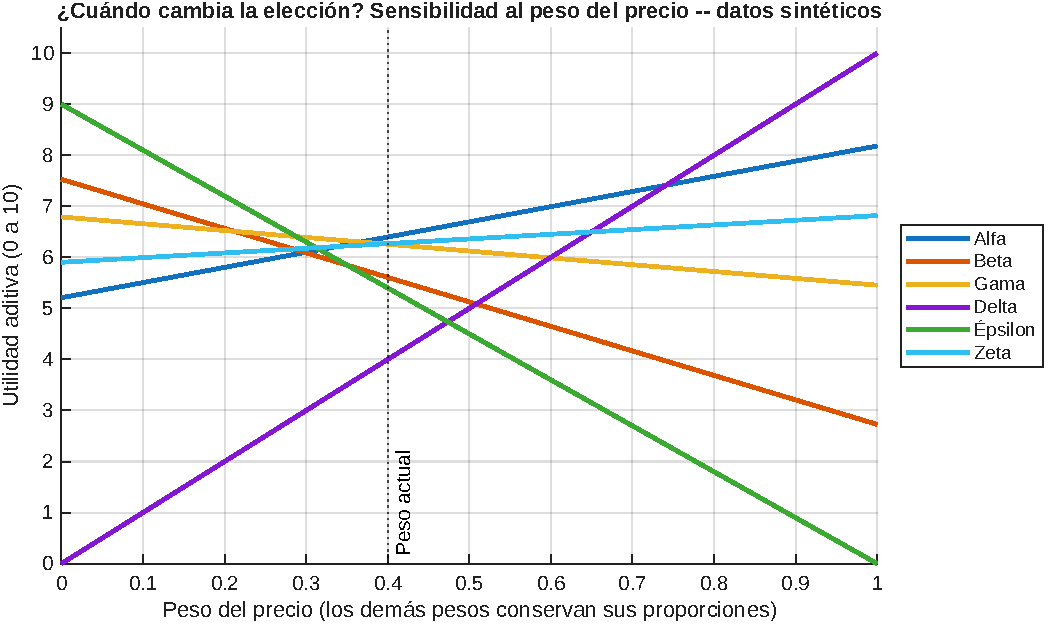
\includegraphics[width=0.88\textwidth]{figuras/matlab/cap06_sensibilidad_peso.pdf}
  \captionof{figure}{Utilidad aditiva de cada alternativa al variar el peso del
  precio. Fuente: elaboración propia con datos sintéticos.}
  \label{fig:cap06-sensibilidad}
\end{center}

\textbf{Interpretación de negocio.} Con los valores por defecto las tres
reglas eligen alternativas distintas: la aditiva elige \textit{Alfa}, la
conjuntiva \textit{Gama} y la lexicográfica \textit{Épsilon}. Ninguna regla
está equivocada. Cada una responde a una pregunta diferente. La aditiva
pregunta qué opción \enquote{rinde más en promedio}. La conjuntiva pregunta
cuál no tiene un defecto inaceptable. La lexicográfica pregunta cuál es mejor
en lo único que de verdad importa. Una marca que ignora esa diferencia
diseña su ficha de producto para una regla y pierde a quienes deciden con
otra.

La figura~\ref{fig:cap06-sensibilidad} agrega una lección de método. La
alternativa elegida por la regla aditiva cambia tres veces al recorrer el
peso del precio de 0 a 1. Una diferencia de pocos centésimos en un peso que
el consumidor declara \enquote{más o menos} basta para cambiar la
recomendación. Los pesos que un modelo infiere o que una encuesta captura
no son constantes físicas.

\textbf{Ejercicio propuesto (usen exactamente este script, solo cambien el
bloque de parámetros).} Corran el script tres veces y completen un cuadro con
la alternativa que elige cada regla y si las tres coinciden:
\begin{enumerate}
  \item \textbf{Caso A — valores por defecto:} los siete parámetros tal como
  están en el script.
  \item \textbf{Caso B — el precio domina:} cambien los pesos a
  \texttt{pesoPrecio = 0.80}, \texttt{pesoCalidad = 0.10},
  \texttt{pesoEntrega = 0.05} y \texttt{pesoResenas = 0.05}, sin tocar nada
  más.
  \item \textbf{Caso C — mínimo exigente:} regresen los pesos a sus valores
  por defecto y cambien \texttt{umbralMinimo} a 6 y
  \texttt{atributoPrioritario} a 3.
\end{enumerate}
Con el cuadro completo, respondan por escrito: en el Caso B, ¿qué
alternativa elige la regla aditiva y por qué la conjuntiva no la acepta? En
el Caso C, ¿qué ocurre con la regla conjuntiva y qué debería hacer el
consumidor? A partir de sus tres corridas, expliquen cuándo conviene usar
primero una regla no compensatoria (para descartar) y después una
compensatoria (para elegir entre las que quedan), y relacionen su respuesta
con lo que \textcite{payne1988adaptive} observaron sobre el esfuerzo de
decisión.

\textbf{Extensión opcional.} Cambien en el script uno de los datos de
\texttt{datosCrudos} (por ejemplo, el precio de \textit{Épsilon}) y
describan cómo se desplaza el punto de cambio de la
figura~\ref{fig:cap06-sensibilidad}.

\textbf{Sin MATLAB.} \texttt{matlab/cap06/cap06\_alternativas\_interactivo.html}
tiene los mismos parámetros, los casos A, B y C, y el cuadro de comparación.

\textbf{Con datos propios (extensión opcional).}
\texttt{cap06\_alternativas\_datos\_propios.html}
aplica las tres reglas a las alternativas y los atributos de un Excel o CSV propio (hoja «Alternativas»; hoja «Criterios» opcional con el tipo y el peso de cada atributo). Permite editar tipos y pesos, cambiar la regla lexicográfica, barrer el peso de un atributo y descargar los resultados. Los datos no salen del navegador.
\end{cajaLaboratorio}

\begin{cajaEtica}
Las tres reglas del laboratorio suponen que el consumidor conoce sus
atributos y sus pesos. En una tienda real, el propio diseño puede moldear
ambas cosas: una insignia, un orden de resultados o un temporizador cambian
qué atributos se vuelven visibles y cuánto pesan. Un equipo de mercadotecnia
que estima \enquote{pesos de preferencia} a partir de clics debe distinguir
la preferencia del consumidor de la respuesta del consumidor a su propia
interfaz. Y toda técnica de urgencia o escasez debe pasar la prueba del
cuadro~\ref{tab:cap06-nudge}: información veraz y una salida tan fácil como
la entrada.
\end{cajaEtica}

\section{Estudio de caso}
\label{sec:cap06-caso}

\begin{casoFicticio}
Una tienda en línea mexicana de electrónicos observa que 7 de cada 10
personas que agregan un producto al carrito lo abandonan. El equipo propone
dos medidas. La primera: un temporizador de 10 minutos con el mensaje
\enquote{tu carrito expira}, que se reinicia cada vez que se recarga la
página. La segunda: una comparación lado a lado con las tres alternativas más
parecidas, que muestra precio real, tiempo de entrega y calificación
promedio con el total de reseñas.

\textbf{Preguntas guía.}
\begin{enumerate}
  \item ¿En qué etapa del proceso de decisión interviene cada medida?
  \item Clasifique cada medida como \textit{nudge} o patrón oscuro con el
  criterio del cuadro~\ref{tab:cap06-nudge} y justifique.
  \item ¿Qué regla de decisión del laboratorio facilita la comparación lado a
  lado? ¿Y cuál obstaculiza el temporizador?
  \item Proponga una métrica distinta de la tasa de conversión inmediata que
  detectaría el costo de la medida manipuladora a mediano plazo.
\end{enumerate}
\end{casoFicticio}

\section{Actividades y evidencias del portafolio}

Esta Parte tiene una sola práctica oficial de 15 horas, \enquote{Recorrido del
consumidor digital}, con un entregable único que se arma en cuatro sesiones
(Cap.~6 a 9). Las actividades de este capítulo producen su primer insumo.

\begin{description}
  \item[Reporte de investigación] Elegir un caso real de compra digital
  (propio o de una persona entrevistada) y describir, etapa por etapa, qué
  ocurrió en cada una de las cinco y qué canal intervino. Señalar si hubo
  reconocimiento inducido. Este caso se retoma en los Cap.~7, 8 y 9.
  \item[Infografía colaborativa] Representar el proceso de decisión de ese
  caso con sus bucles y retrocesos (figura~\ref{fig:cap06-proceso} como
  punto de partida, no como plantilla obligatoria).
  \item[Solución de casos] Resolver por escrito el estudio de caso de la
  tienda de electrónicos (sección~\ref{sec:cap06-caso}).
  \item[Reporte de práctica] Incluir el cuadro de los tres casos del
  ejercicio propuesto del laboratorio (sección~\ref{sec:cap06-lab}) con las respuestas a las
  preguntas de comparación. Se integra al entregable único de la práctica
  \enquote{Recorrido del consumidor digital} (ver \enquote{Prácticas
  oficiales de la unidad} al cierre de esta Parte).
\end{description}

\section{Ruta de aprendizaje autónomo}

Dos horas de aprendizaje autónomo. Tareas concretas:
\begin{enumerate}
  \item Ejecutar \texttt{cap06\_alternativas\_interactivo.html} y completar
  el cuadro de los casos A, B y C.
  \item Navegar una tienda en línea que usen con frecuencia y registrar tres
  elementos de interfaz que activen escasez, urgencia o prueba social.
  Clasificar cada uno con el cuadro~\ref{tab:cap06-nudge}.
  \item Entrevistar a una persona sobre una compra reciente y ubicar en las
  cinco etapas lo que relata (insumo del reporte de investigación).
  \item (Opcional) Con \texttt{cap06\_alternativas\_datos\_propios.html} (opcional), evaluar \textbf{sus propias alternativas} (por ejemplo, tres opciones reales del caso del equipo) y escribir en dos líneas si las tres reglas coinciden.
\end{enumerate}

\section{Síntesis}

El proceso de decisión de compra tiene cinco etapas: reconocimiento,
búsqueda, evaluación, decisión y evaluación post-compra. En internet, el
orden se tuerce. El reconocimiento puede ser inducido por el algoritmo, la
búsqueda mezcla fuentes de la marca, de terceros y sociales, la decisión
regresa a evaluar y la reseña propia alimenta la búsqueda ajena. En la etapa
de evaluación, las personas rara vez ponderan todo. Usan reglas compensatorias
cuando las alternativas son pocas y no compensatorias cuando son muchas, y la
regla elegida puede cambiar el producto elegido. La interfaz es una
arquitectura de elección: usada con información veraz es un \textit{nudge};
usada para mentir o impedir la salida, es un patrón oscuro.

\subsection*{Glosario del capítulo}
\begin{description}
  \item[Arquitectura de elección] Forma en que se presentan las opciones a quien decide (orden, valores por defecto, información visible).
  \item[Atributo de costo] Atributo en el que un valor menor es mejor (precio, días de entrega).
  \item[Atributo prioritario] Parámetro editable que indica por cuál atributo empieza la regla lexicográfica: 1 precio, 2 calidad, 3 entrega, 4 reseñas. Rango: entero de 1 a 4.
  \item[Heurística] Atajo de juicio que sustituye el cálculo exhaustivo cuando la información es abundante o incierta.
  \item[Nudge] Modificación del contexto de decisión que no prohíbe opciones ni cambia incentivos de forma significativa.
  \item[Patrón oscuro (\textit{dark pattern})] Diseño de interfaz que engaña o presiona para que la persona decida algo que no habría decidido con información veraz y una salida fácil.
  \item[Peso de un atributo] Parámetro editable (\texttt{pesoPrecio}, \texttt{pesoCalidad}, \texttt{pesoEntrega}, \texttt{pesoResenas}) que expresa su importancia. Rango: real $\ge 0$, con al menos un peso mayor que 0; el script los normaliza. Los casos didácticos usan valores entre 0.05 y 0.80.
  \item[Reconocimiento inducido] Necesidad percibida que genera el canal (notificación, recomendación) sin que exista una carencia previa.
  \item[Regla compensatoria] Regla en la que un atributo bueno puede compensar uno malo.
  \item[Regla no compensatoria] Regla en la que un atributo malo (conjuntiva) o poco prioritario (lexicográfica) no puede compensarse con otros.
  \item[Tolerancia lexicográfica] Parámetro editable: diferencia, en puntos de la escala 0--10, que se considera empate. Rango: real entre 0 y 10; los casos didácticos usan valores entre 0 y 1.5.
  \item[Umbral mínimo] Parámetro editable de la regla conjuntiva: puntaje mínimo (0 a 10) exigido en cada atributo. Rango: real entre 0 y 10; los casos didácticos usan valores entre 3.5 y 6.
  \item[\textit{Webrooming} / \textit{showrooming}] Investigar en línea y comprar en tienda / probar en tienda y comprar en línea.
\end{description}

\subsection*{Autoevaluación}

\textbf{Opción múltiple}

\begin{enumerate}
  \item El \enquote{reconocimiento inducido} se distingue del reconocimiento
  clásico porque:
  \begin{enumerate}
    \item[a)] Ocurre solo en tiendas físicas.
    \item[b)] La brecha percibida nace del diseño del canal y no de una carencia previa de la persona. \textit{(correcta)}
    \item[c)] Elimina la etapa de búsqueda de información.
    \item[d)] Solo aplica a productos de lujo.
  \end{enumerate}
  \textit{Justificación:} subsección 5.2.1.

  \item Una alternativa con el mejor precio pero el peor puntaje de calidad
  puede ganar con la regla aditiva y quedar fuera con la conjuntiva porque:
  \begin{enumerate}
    \item[a)] La regla aditiva ignora el precio.
    \item[b)] La aditiva permite que un atributo compense a otro; la conjuntiva exige un mínimo en cada uno. \textit{(correcta)}
    \item[c)] La conjuntiva solo mira el precio.
    \item[d)] Las dos reglas siempre coinciden.
  \end{enumerate}
  \textit{Justificación:} sección~\ref{sec:cap06-evaluacion} y laboratorio.

  \item Un temporizador de \enquote{expira en 10 minutos} que se reinicia al
  recargar la página es, según el criterio del capítulo:
  \begin{enumerate}
    \item[a)] Un \textit{nudge}, porque acelera la compra.
    \item[b)] Un patrón oscuro, porque la urgencia es falsa. \textit{(correcta)}
    \item[c)] Una regla lexicográfica.
    \item[d)] Un dato de primera parte.
  \end{enumerate}
  \textit{Justificación:} recuadro de Frontera de la sección~\ref{sec:cap06-evaluacion} y cuadro~\ref{tab:cap06-nudge}.
\end{enumerate}

\textbf{Preguntas abiertas}

\begin{enumerate}
  \item Explique por qué asignar a una persona la etiqueta \enquote{comprador
  en línea} describe una compra y no una identidad. \textit{Clave:} debe
  mencionar el \textit{webrooming} y el \textit{showrooming} y que dependen de
  la categoría de producto (sección~\ref{sec:cap06-busqueda}).
  \item A partir de la figura~\ref{fig:cap06-sensibilidad}, explique qué
  implica para un equipo de mercadotecnia que la alternativa elegida cambie
  al variar poco el peso del precio. \textit{Clave:} los pesos estimados no
  son constantes; la recomendación debe acompañarse de un análisis de
  sensibilidad y no de un número único.
\end{enumerate}

\section{Lecturas recomendadas}

\begin{description}
  \item[\textcite{simon1955}] El artículo breve en que la elección \enquote{suficientemente buena} sustituye a la óptima. Se lee en una tarde y explica por qué el laboratorio incluye reglas no compensatorias.
  \item[\textcite{payne1988adaptive}] Muestra que las estrategias de decisión se adaptan al esfuerzo que exigen. Es la base empírica del contraste entre reglas del capítulo.
  \item[\textcite{mathur2019}] Estudio empírico de patrones oscuros en miles de sitios de compra. Útil para entrenar el ojo antes del ejercicio de la ruta autónoma.
  \item[\textcite{thalersunstein2008}] Obra de divulgación que popularizó el \textit{nudge}. Léase junto con \textcite{thaler2003libertarian}, su antecedente arbitrado.
\end{description}
